\begin{figure}
  \centering 
  \begin{subfigure}[b] 
{0.45\textwidth}
    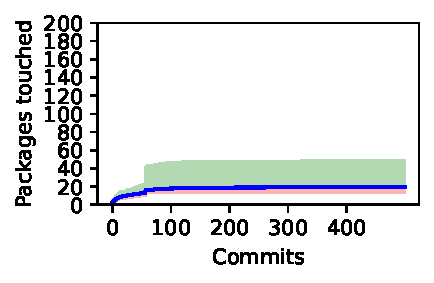
\includegraphics{sections/results/14/packages/time_series_components_touched.packages.all.founders.commits_500.pdf}
    \caption{Packages for All founders (n=29, $\mu$=19.45, median=6.0 \& std=25.32)}
    \label{figure.sections/results/14/packages/time_series_components_touched.packages.all.founders.commits_500.pdf}
  \end{subfigure}
  \begin{subfigure}[b] 
{0.45\textwidth}
    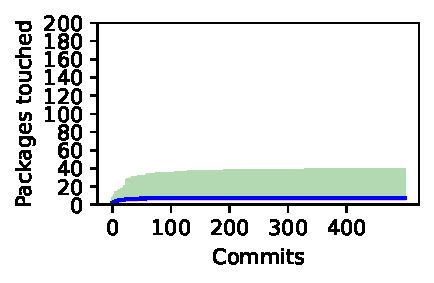
\includegraphics{sections/results/14/packages/time_series_components_touched.packages.all.joiners.commits_500.pdf}
    \caption{Packages for All joiners (n=637, $\mu$=7.75, median=2.0 \& std=16.58)}
    \label{figure.sections/results/14/packages/time_series_components_touched.packages.all.joiners.commits_500.pdf}
  \end{subfigure}
\newpage 
  \begin{subfigure}[b] 
{0.45\textwidth}
    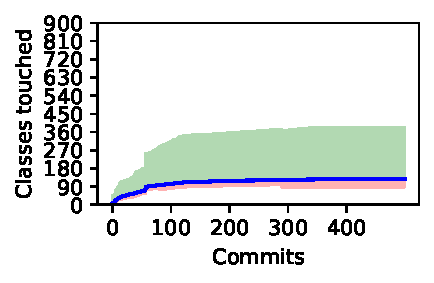
\includegraphics{sections/results/14/classes/time_series_components_touched.classes.all.founders.commits_500.pdf}
    \caption{Classes for All founders (n=29, $\mu$=125.62, median=13.0 \& std=198.53)}
    \label{figure.sections/results/14/classes/time_series_components_touched.classes.all.founders.commits_500.pdf}
  \end{subfigure}
  \begin{subfigure}[b] 
{0.45\textwidth}
    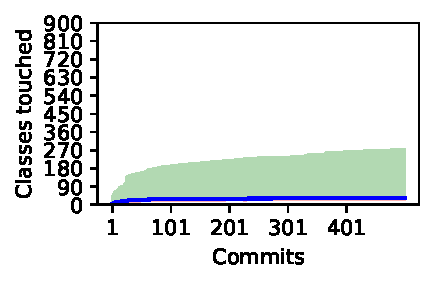
\includegraphics{sections/results/14/classes/time_series_components_touched.classes.all.joiners.commits_500.pdf}
    \caption{Classes for All joiners (n=637, $\mu$=31.25, median=1.0 \& std=96.12)}
    \label{figure.sections/results/14/classes/time_series_components_touched.classes.all.joiners.commits_500.pdf}
  \end{subfigure}
\newpage 
  \begin{subfigure}[b] 
{0.45\textwidth}
    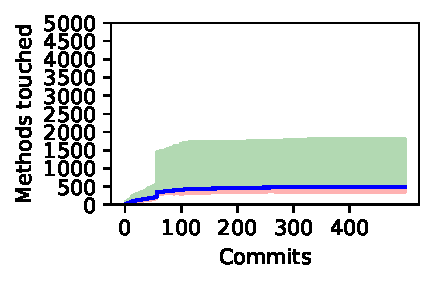
\includegraphics{sections/results/14/methods/time_series_components_touched.methods.all.founders.commits_500.pdf}
    \caption{Methods for All founders (n=29, $\mu$=494.48, median=52.0 \& std=910.58)}
    \label{figure.sections/results/14/methods/time_series_components_touched.methods.all.founders.commits_500.pdf}
  \end{subfigure}
  \begin{subfigure}[b] 
{0.45\textwidth}
    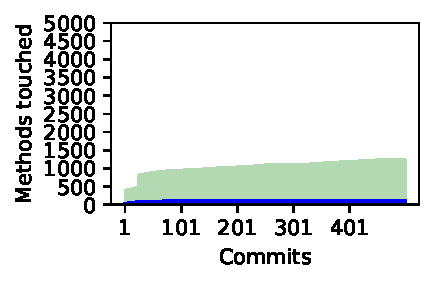
\includegraphics{sections/results/14/methods/time_series_components_touched.methods.all.joiners.commits_500.pdf}
    \caption{Methods for All joiners (n=637, $\mu$=111.15, median=1.0 \& std=427.09)}
    \label{figure.sections/results/14/methods/time_series_components_touched.methods.all.joiners.commits_500.pdf}
  \end{subfigure}
\caption{Repository 14 A time series for the all commits, excluding transient, with the average mean (blue line), all components touched (y-axis) against the number of commits (x-axis) for six (6) developer categories. Green is the standard deviation above the mean, and pink is the standard deviation below the mean.}\end{figure}
\clearpage 
\newpage 
